\documentclass[a4paper,11pt]{article}
\usepackage[a4paper, left=1.5cm, right=1.5cm, top=2.0cm, bottom=3.5cm, headsep=1.2cm]{geometry}
\usepackage{polski}
\usepackage{amssymb}
\usepackage[utf8]{inputenc}
\prefixing
\usepackage{latexsym}
\usepackage{graphicx}
\usepackage{hyperref}
\author{Klaudia Balcer}
\title{Testowanie wielokrotne}
\frenchspacing
\begin{document}
\maketitle
\begin{center}
Zaawansowane Modele Liniowe

Raport 5
\end{center}
\tableofcontents

\pagebreak
\section*{Wstęp}

Pomiary wielokrotne łamią jedno z podstawowych, obecnych dotychczas wszędzie, założeń -- nie zakładamy w tym modelu niezależności obserwacji.  Zakładamy jednakże liniową zależność między zmiennymi objaśnianą (będź pewną jej funckją zwaną linkującą) a objaśniającymi.

Odpowiada to często spotykanym w rzeczywistości sytuacjom typu badanie własności obiektu w czasie (np. waga pacjenta w trakcie kuracji).  

W poniższym sprawozdaniu przedstawię symulację ze zmienną objaśniającą z rozkładu normalnego i funckją identycznościową jako funckją linkującą.  

Kowariancje między wartościami targetu w kolejnych obserwacjach dla jednego parametru opisane zostaną macierzą $\Sigma$; zmienne odpowiedzi dla obserwacji odpowiadających róznym obiektom są  niezależne. Zmienne objaśniające będę generować z rozkładu normalnego.  Następnie będę symulować Y-ki im odpowiadające z wielowymiarowego rozkładu normalnego o średniej $X\beta$  i wariancji $Sigma$,  model i estymatory kolejnych parametrów  500-krotnie. Do implementacji modelu opisanego powyżej użyję funkcji gls() z pakietu nlme.

\section{Generowanie danych i estymacja parametrów dla jednej symulacji}
Macierz opisująca kowariancję między $y_{i}$ dla ustalonego obiektu:

\begin{center}

$\Sigma = $
\left(\begin{array}{ccc}
4 & 1.2 &  1.2 \\
1.2 &  4 &  1.2 \\
1.2 &  1.2  & 4 \\
\end{array}\right)
$ = \gamma^{2}$
\left(\begin{array}{ccc}
1 & \rho & \rho \\
\rho & 1 & \rho \\
\rho & \rho & 1 \\
\end{array}\right)

\end{center}

Estymator macierzy $\Sigma$ uzyskany z modelu za  pomocą funckji getVarCov():

\begin{center}

$\widehat{\Sigma} = $
\left(\begin{array}{ccc}
4.8028 & 1.2377 &  1.2377 \\
1.2377 &  4.8028 &  1.2377 \\
1.2377 &  1.2377  & 4.8028 \\
\end{array}\right)

\end{center}

co daje estymatory parametrów $\rho$ i $\gamma$:

$\widehat{\rho} = 0.2577071$,$\quad ||\widehat{\rho} -\rho||_{sup} =  0.04229294$, $ \quad\widehat{\gamma} =  2.191529 $, $\quad || \widehat{\gamma} - \gamma||_{sup} = 0.191529 $


Mając estymator macierzy kowariancji mogę przystąpić do estymacji wektora współczynników regresji\footnote{wektor $\beta$ można \textit{wyciągnąć} wprost z modelu, a tym sprawozdaniu jednak wykorzystamy jego analityczną postać}. Estymator $\beta =  (0, 3,  3, 0)'$ dany jest wzorem i daje wyniki:

\begin{center}

$\widehat{\beta} = \Bigg(\sum_{i=1}^{n} X'_{i}\widehat{\Sigma}^{-1}X_{i}\Bigg)^{-1}\Bigg(\sum_{i=1}^{n} X'_{i}\widehat{\Sigma}^{-1}y_{i}\Bigg)$
$ =$ \left(\begin{array}{c}
0.3687285 &  2.3059417 &  0.6389446 & -0.2846345
\end{array}\right)

\end{center}

z normą supremum obciążenia:
$\quad || \beta - \widehat{\beta}||_{sup} = 2.361055 $

Podobnie macierz kowariancji estymatora wektora współczynników regresji liniowej możemy wyciągnąc wprost z modelu lub wyliczyć ze wzoru (macierz będąca pierwszym cżłonem wzoru na estymator $\widehat{\beta}$ jest wzorem na macierz kowariancji $\widehat{\beta}$). 

Macierz kowariancji beta wyliczona ze wzoru z użyciem macierzy $\Sigma$ (prawdziwa wartość kowariancji między $y_{i}$):

\begin{center}

$cov(\widehat{\beta}) = $ \left(\begin{array}{cccc}
 0.11108656 & -0.05232137  & -0.1048936 & -0.02273040 \\
-0.05232137 &   3.34907494 &  -0.4392636 &  -0.07034852 \\
-0.10489360 &  -0.43926360  &  3.5245946  &  0.76502953\\
-0.02273040  & -0.07034852 &   0.7650295  &  2.73119729\\
\end{array}\right)

\end{center}

Macierz kowariancji beta wyliczona ze wzoru z użyciem macierzy $\widehat{\Sigma}$ (wyestymowana przez model wartość kowariancji między $y_{i}$):

\begin{center}

$cov(\widehat{\beta})=$\left(\begin{array}{cccc}
 0.12675186  & -0.06515689  & -0.1288785 &  -0.02710482 \\
-0.06515689  &  4.15972526 &  -0.5400588  & -0.05149201 \\
-0.12887850 &  -0.54005876  &  4.3304419   & 0.89316833 \\
 -0.02710482 &  -0.05149201 &   0.8931683  &  3.38614241  \\
\end{array}\right)

\end{center}

norma supremum  obciążenia tej estymacji:  0.8106503

Wyliczona ze wzoru macierz przystaje z macierzą uzyskaną z modelu za pomocą funkcji vcov().

\section{Rozkłady uzyskanych estymatorów}
\subsection{n=20, p=4,  k=3,  method = 'REML'}
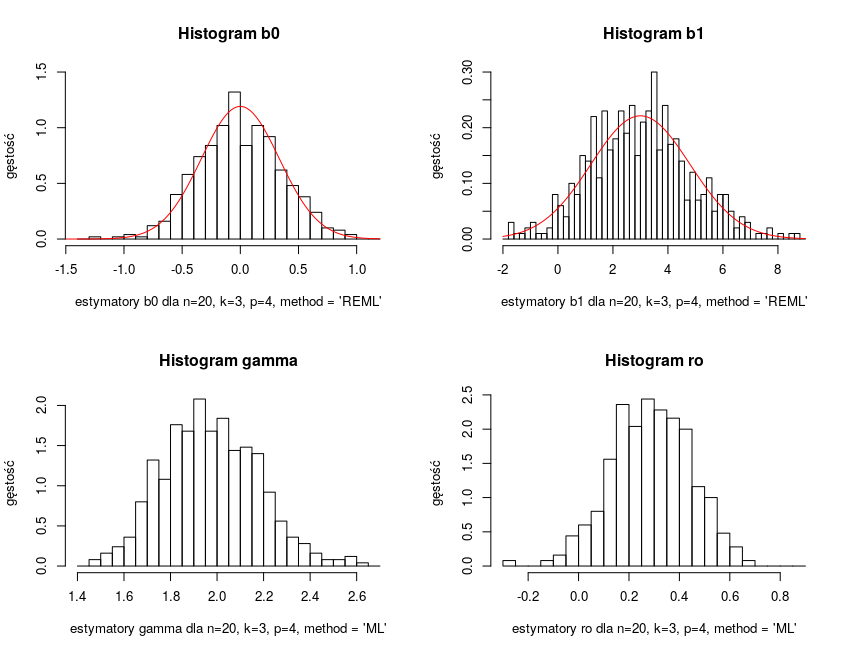
\includegraphics[scale=.8]{Rplot2.png} 

\subsection{n=100, p=4,  k=3,  method = 'REML'}
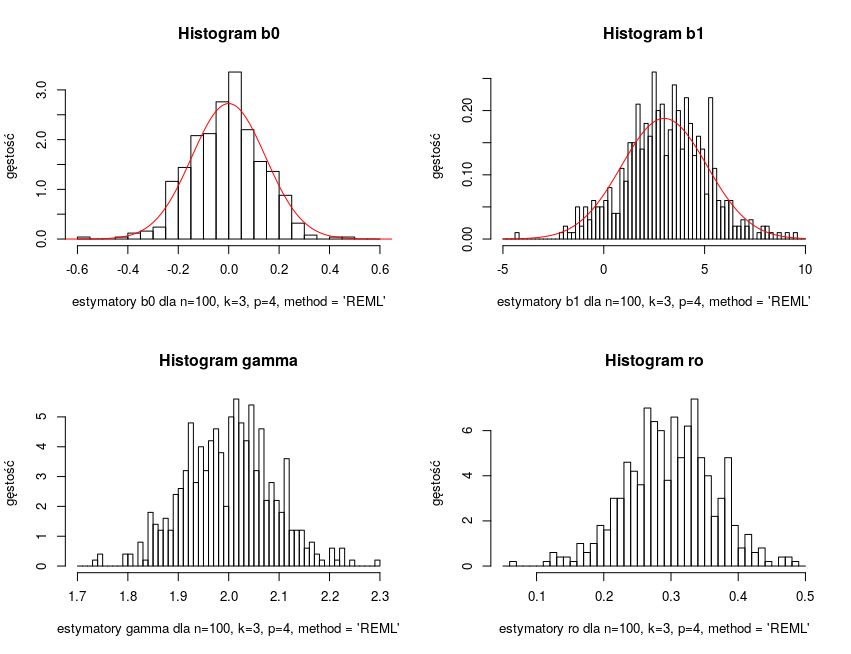
\includegraphics[scale=.8]{Rplot3.png} 

\subsection{n=100, p=4,  k=15,  method = 'REML'}
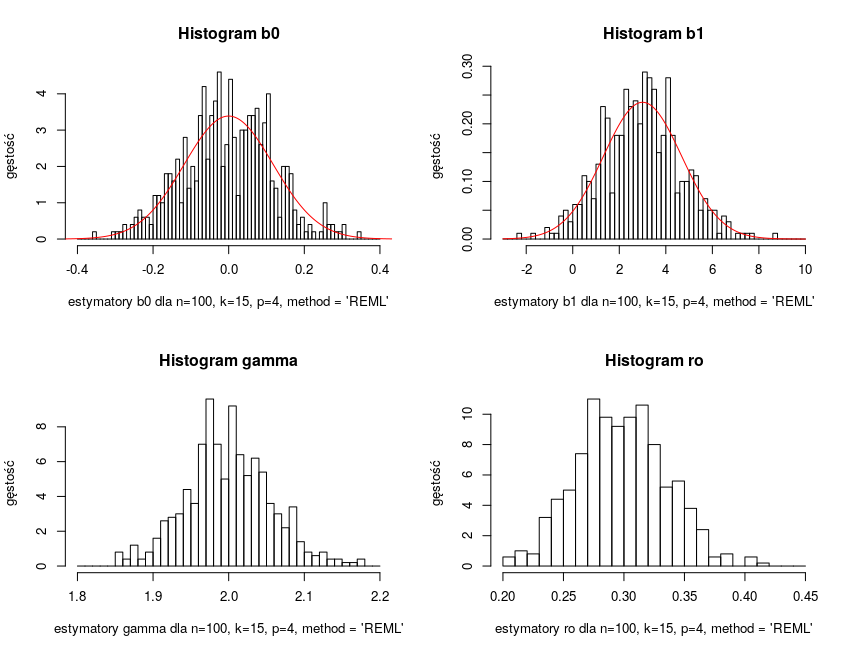
\includegraphics[scale=.8]{Rplot4.png} 

\subsection{n=100, p=4,  k=20,  method = 'REML'}
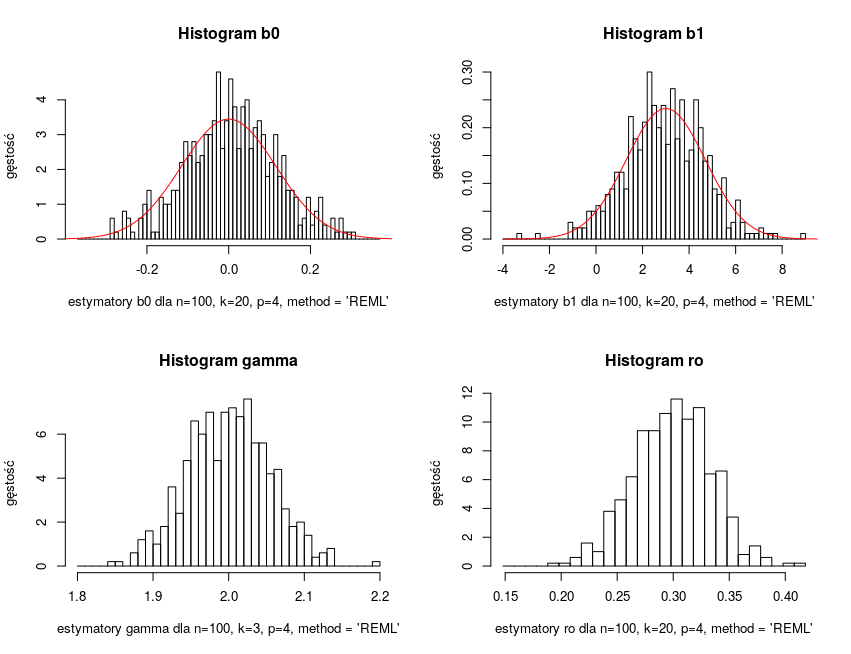
\includegraphics[scale=.8]{Rplot5.png} 

\subsection{n=20, p=4,  k=3,  method = 'ML'}
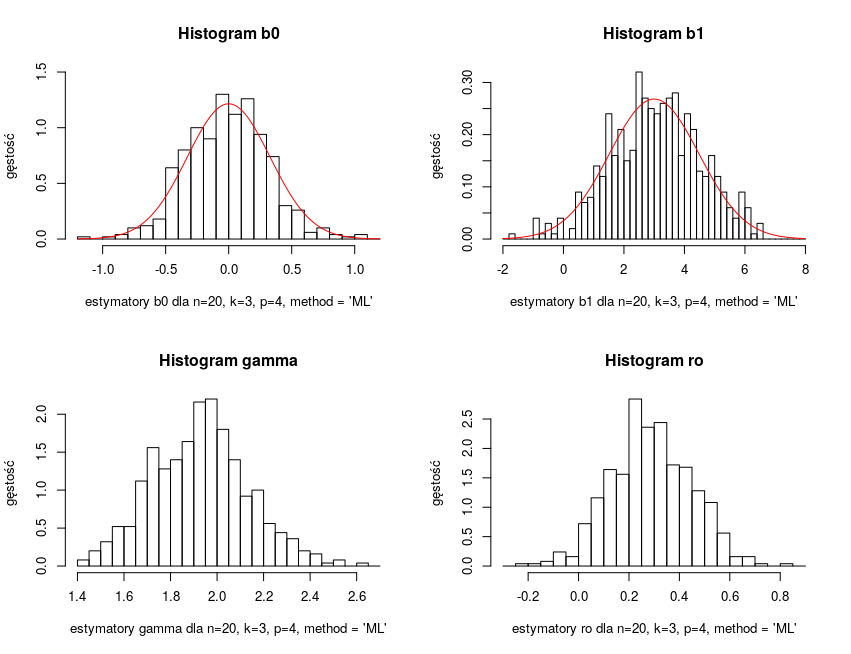
\includegraphics[scale=.8]{Rplot62.png} 

\subsection{n=100, p=4,  k=3,  method = 'ML'}
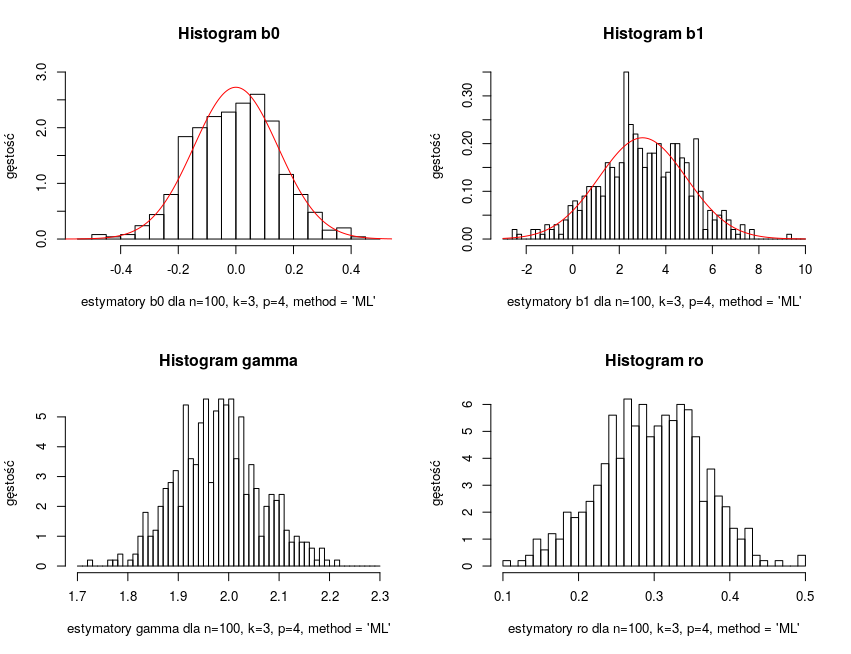
\includegraphics[scale=.8]{Rplot63.png} 

\subsection{n=100, p=4,  k=15,  method = 'ML'}
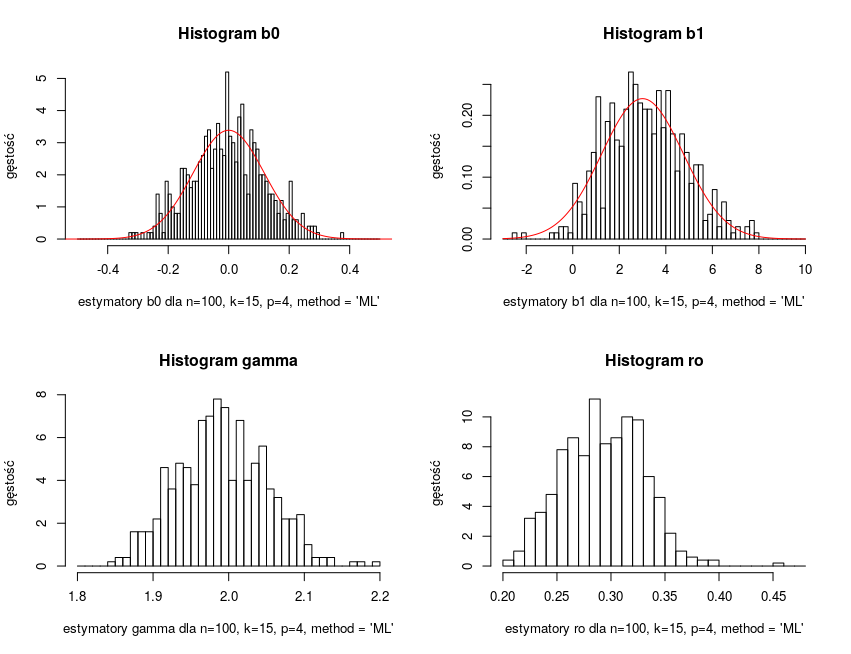
\includegraphics[scale=.8]{Rplot64.png}

\subsection{n=100, p=4,  k=20,  method = 'ML'}
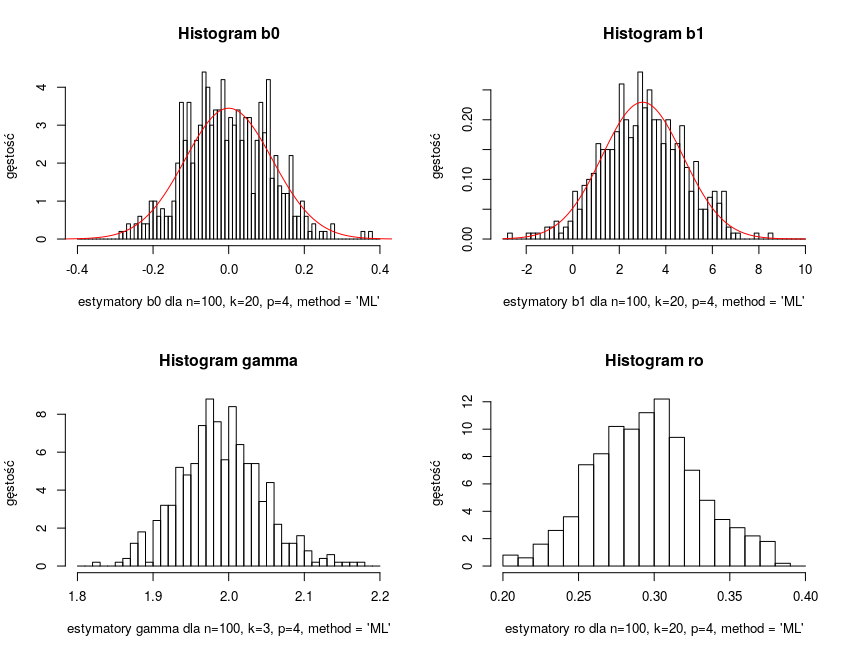
\includegraphics[scale=.8]{Rplot65.png} 

\subsection{Obciążenia estymatorów i norma  supremum \beta}

\begin{center}
\begin{tabular}{|c|c|c|c|c|c|c|c|} \hline

 przykład & $bias(\widehat{\beta_{0}})$ &   $bias(\widehat{\beta_{1}})$  &   $bias(\widehat{\beta_{2}})$   &  $bias(\widehat{\beta_{3}})$  &  $bias(\widehat{\gamma})$  &   $bias(\widehat{\rho})$   & $ ||\beta - \widehat{\beta}||_{sup}$ \\ \hline
1 & 0.2854076  &1.4502871  & 1.3663709  & 1.4864994 &  0.1662176  & 0.1276397  & 2.3390187 \\
  2&
0.11043018  & 1.61513885  & 1.53710592  & 1.48866924  & 0.07014821  & 0.05233165  & 2.61168729  \\
3 &
0.09524312  & 1.32182196  & 1.37860940  & 1.36089407  & 0.04449272  & 0.02978171  & 2.26547747 \\
4 &
0.08910844 &  1.35283211  & 1.31915900  & 1.36861566  & 0.04387761  & 0.02757252  & 2.27275779 \\
5 &
 0.2561832   & 1.2014324   & 1.3334717   & 1.7947791   & 0.1743675   & 0.1289453   & 2.4520189 \\
 6 &
0.12009840  & 1.52817520  & 1.49806126  & 1.49836296  & 0.06787157  & 0.05355533  & 2.49933586 \\
7 &
0.09586099  & 1.37835260  & 1.36982080  & 1.34527067  & 0.04841068  & 0.03088703  & 2.24006547  \\
8 &
0.08822373  & 1.40755279  & 1.38615623  & 1.29766260  & 0.04411836  & 0.02847026  & 2.31381621 \\ \hline

\end{tabular}
\end{center}

\section{Wnioski:}

Przyrost n lub k poprawia estymację parametrów. Innymi słowy wzrost liczby badanych obiektów (n) lub ilość pomiarów wykonanych dla każdego obiektu (k) przyczynia się do polepszenia estymacji (obie te liczby przekładają się liniowo na ilość obserwacji w modelu, stąd naturalnym wydaje się wniosek że  estymacja jest dokładniejsza, gdy jest ich więcej).

 Lepsze rezultaty obserwujemy dla metody REML.

\section{Implementacja symulacji}

\begin{verbatim}
library(mvtnorm)
library(nlme)
corr<- corCompSymm(form=~1|id)
wei  <-  varIdent(form=~1)

generate_X <- function(n, k, p){
  matrix(rnorm(n*k*(p-1), 0, 1/sqrt(n*k)),  n*k, p-1)
}

generate_sigma <- function(n, k, p){
  sigma <- matrix(rep(ro, k^2), k, k)
  diag(sigma) <- rep(1, k)
  sigma <- sigma  * gama^2
}

generate_Y <-  function(n, k, p,  X, sigma){
  Y <- as.vector(sapply(seq(n), function(i){
    Xbeta <-  matrix(1, k,  p)
    Xbeta[,2:p] <- X[seq((i-1)*k+1,i*k), ]
    Xbeta <-  Xbeta%*%beta
    rmvnorm(1, Xbeta, sigma)}))
  id <-  as.vector(sapply(seq(n), function(i)(rep(i, k))))
  Tvec <-  rep(seq(k), n)
  data.frame(Y, id, Tvec, X0=rep(1,  n*k), X)
}

cov_beta <- function(sigma_est1, n=20, k=3, p=4, dataf){
  id <- seq(n)
  res1 <- matrix(rep(0), p, p)
  for(i in id){
    x <- dataf[which(dataf$id==i),4:(p+3)]
    res1 <- res1 + t(as.matrix(x))%*%sigma_est1%*%as.matrix(x)
  }
  solve(res1)
}

generate_estimators <- function(n, k, p,  X, sigma){
  dataf <- generate_Y(n, k, p,  X, sigma)
  mod1 <- gls(Y~.-id -Tvec -X0, dataf, corr, wei, method="REML")
  sigma_est <-  getVarCov(mod1)
  s <- solve(sigma_est)
  res2 <- rep(0, p)
  for(i in seq(n)){
    x <- dataf[dataf$id==i,4:(p+3)]
    res2 <- res2 + t(x)%*%s%*%dataf$Y[dataf$id==i]
  }
  cov_beta_est <-  cov_beta(s, n, k, p, dataf)
  beta_est <- cov_beta_est%*%res2
  est_gamma  <- sqrt(diag(sigma_est)[1])
  est_ro <-  sigma_est[1,2]/diag(sigma_est)[1]
  real_beta_cov <- cov_beta(solve(sigma), n, k, p, dataf)
  c(beta_est, est_gamma, est_ro, real_beta_cov[1,1], real_beta_cov[2,2])
}

generate_results <- function(n, k, p, times=500){
  X <-  generate_X(n=n, k=k, p=p)
  sigma <-  generate_sigma(n, k, p)
  sapply(rep(n, times), generate_estimators, k, p,  X, sigma)
}

set.seed(128)
ro <- 0.3
gama <- 2
beta <- c(0, 3, 3, 0)

# Zad 2
par(mfrow=c(2,2))

z2 <- generate_results(n=20, k=3, p=4)
hist(z2[1,], main = "Histogram b0", freq=F, ylab = 'gęstość', 
xlab = "estymatory b0 dla n=20, k=3, p=4, method = 'REML'", ylim=c(0, 1.5), 
breaks = seq(-1.4, 1.2, 0.1))
lines(seq(-1.5, 1.2, 0.001), dnorm(seq(-1.5, 1.2, 0.001), 0, 
sqrt(z2[7,1])), col=2)
hist(z2[2,], main = "Histogram b1", freq=F, ylab = 'gęstość', 
xlab = "estymatory b1 dla n=20, k=3, p=4, method = 'REML'", breaks = seq(-2, 9, .2))
lines(seq(-2, 9, 0.01), dnorm(seq(-2, 9, 0.01), 3, sqrt(z2[8,1])), col=2)
hist(z2[5,], main = "Histogram gamma", freq=F, ylab = 'gęstość', 
xlab = "estymatory gamma dla n=20, k=3, p=4, method = 'ML'", breaks = seq(1.4, 2.7,  0.05))
hist(z2[6,], main = "Histogram ro", freq=F, ylab = 'gęstość',
 xlab = "estymatory ro dla n=20, k=3, p=4, method = 'ML'", breaks = seq(-.3, .9, 0.05))

\end{verbatim}

\end{document}